\capitulo{4}{Técnicas y herramientas}

Para el desarrollo del presente proyecto se utilizaron diferentes técnicas, herramientas y software, de los cuales es necesario precisar algunos conceptos. Es importante mencionar que, la decisión de implementar o utilizar un software, técnica o herramienta en particular, y no otra, se tomó con base a la valoración realizada en cada caso, y que se incluye en este apartado a modo de justificación.

\subsection{Entorno software}

\subsubsection{Golang}

El backend desarrollado en el presente proyecto se basó en el lenguaje Golang, también conocido como Go, que es un lenguaje de programación de código abierto desarrollado por Google en 2007, y que se utiliza principalmente para aplicaciones de sistemas, redes y servicios web. Go presenta una serie de ventajas que permiten a los programadores ser más productivos, por ejemplo: su rendimiento, modelo de concurrencia, seguridad, portabilidad y facilidad de aprendizaje, razones por las que fue elegido para este proyecto \cite{book:golang_donovan}.

En este sentido, y frente a alternativas como Java o Rust, Golang es más rápido debido a su compilación estática, lo que significa que el código se compila antes de que se ejecute, además, utiliza una recolección de basura eficiente, por lo que los recursos del sistema se administran de manera más adecuada. Asimismo, Golang tiene un modelo de concurrencia incorporado que permite crear aplicaciones que pueden manejar múltiples tareas al mismo tiempo sin afectar el rendimiento \cite{book:golang_programacion}. 

Por otro lado, Golang es un lenguaje compilado, por lo que consume muy pocos recursos como espacio en disco y memoria RAM, lo que permite que, incluso en un servidor de poca capacidad, se pueda manejar una gran cantidad de peticiones HTTP. Al mismo tiempo, este lenguaje de programación es compatible con múltiples plataformas, sin tener que realizar cambios significativos en el código, siendo a su vez fácil de aprender por su sintaxis simple y concisa \cite{book:golang_programacion}, lo que concuerda con los objetivos planteados. Finalmente, es importante destacar que en la selección del lenguaje Golang influyó también la familiaridad previa que se tenía con éste por su uso frecuente en el entorno laboral.

\subsubsection{Python}
De igual forma, también se utilizó Python para el desarrollo del Chatbot. Python es un lenguaje de programación de alto nivel, orientado a objetos, que presenta una gran cantidad de características similares con otros lenguajes como C++, Java, Modula-3 y Scheme, por lo que ofrece un equilibrio óptimo entre lo práctico y lo conceptual. Viene con una gran biblioteca de módulos que se pueden utilizar en amplia variedad de tareas que van desde el desarrollo web a gráficos, e incluso inteligencia artificial \cite{book:mckinney_python} \cite{book:mitchell_r}. 

Por otro lado, Python es un lenguaje interpretado, debido a que los programas desarrollados en éste se ejecutan a través de un intérprete. En tanto, una de las grandes ventajas que ofrece Python es su fácil por su sintaxis simple, clara y concisa que facilita su aprendizaje y el mantenimiento de proyectos de gran envergadura, al mismo tiempo que ofrece un entorno multiplataforma que puede ser ejecutado en diversos sistemas operativos \cite{book:mitchell_r}.

\subsection{Control de datos}

\subsubsection{PostgreSQL}
PostgreSQL es un sistema de gestión de bases de datos, de tipo relacional, de código abierto y gratuito. Es considerado uno de los sistemas de bases de datos más potentes y complejos disponibles en el mercado. Entre las aplicaciones de PostgreSQL se encuentran la gestión de datos financieros, sistemas de información geográfica, aplicaciones, y la gestión de datos de grandes empresas. PostgreSQL funciona mediante la ejecución de consultas SQL que permiten la creación, modificación y eliminación de datos almacenados en la base de datos.

Dentro de las ventajas de PostgreSQL, que representan la razón de su elección, se incluyen: a) su potencia y fiabilidad \cite{book:momjian_b}; b) ofrece una amplia gama de características avanzadas, como la replicación y la partición de datos \cite{book:Obe}; c) es compatible con una amplia variedad de lenguajes de programación, como Golang, y sistemas operativos \cite{book:fontaine}; d) es fácil de extender y personalizar mediante el uso de complementos y módulos adicionales \cite{book:schoning}; y e) es de código abierto y gratuito, lo que favorece positivamente el aspecto económico del proyecto \cite{book:momjian_b}.

\subsubsection{Scrapping}
Scrapping es una técnica de extracción de información de páginas web, de manera automática, que permite recopilar una gran cantidad de datos en poco tiempo \cite{book:rusell}, que pueden ser útiles en ámbitos tan diversos que van desde el análisis de mercado hasta la investigación científica. Esta técnica consiste en programar un software que analiza el código HTML de la página web y extrae la información deseada \cite{book:rusell}.

\subsubsection{Postman}
Postman es una herramienta de prueba de APIs moderna que permite a los desarrolladores crear, probar, documentar y compartir APIs de manera rápida y fácil \cite{art:bhattacharya}. En ella, los desarrolladores pueden crear solicitudes HTTP personalizadas y enviarlas a cualquier API en línea o local, y de varias formas, incluyendo los métodos GET, POST, PUT, DELETE y PATCH, lo que permite ahorrar tiempo y recursos \cite{art:chatterjee}. En este sentido, se seleccionó esta herramienta para el presente proyecto por ser gratuita, por la facilidad que ofrece para hacer pruebas de test funcionales sobre APIs antes de implementarlas en el desarrollo de su versión móvil, y por permitir ejecutar pruebas automatizadas sobre las APIs, mediante el uso de Runners.

\subsubsection{Swagger}
Swagger hace referencia a un conjunto de herramientas, especificaciones y reglas destinadas a la documentación de las APIs, y que viene a resolver los problemas generados por la falta de estandarización en el diseño de las mismas. Su principal ventaja es que es fácil de utilizar dada su simplicidad, y que la documentación generada puede implementarse directamente en la automatización de procesos dependientes de APIs. Por otra parte, Swagger permite hacer pruebas de APIs, y sus elementos, al mismo tiempo que muestra los endpoints del proyecto \cite{art:swagger_lopez}. Entonces, Swagger ayuda a describir, producir, consumir y visualizar APIs RESTful para que cualquier desarrollador pueda entender y utilizarlas \cite{art:swagger_rodriguez}.

\subsubsection{FAISS}
FAISS es un biblioteca destinada a la búsqueda de documentos similares a otro documento de consulta, en una base de datos de vectores. Permite personalizar la participación de la base de datos, la codificación y el preprocesamiento de los vectores, para que el conjunto de datos pueda guardarse en la RAM. En este sentido, dentro del presente proyecto FAISS se utilizó para crear vectores de búsqueda de información para crear las respuestas para el chatbot \cite{art:faiss}

\subsection{Infraestructura}

\subsubsection{Docker}
En base a la información previamente explicitada respecto de Docker, se optó por el uso de sus contenedores ya que permiten la creación de entornos de desarrollo aislados y reproducibles, mejorando así la eficiencia del desarrollo de software. 

\subsubsection{Docker Hub}
Docker Hub es un repositorio en la nube, público, para imágenes de contenedores de soluciones prediseñadas de los usuarios de la plataforma Docker. Permite almacenar, administrar, compartir y utilizar imágenes proporcionadas por proveedores oficiales o externos. En este sentido, Docker Hub es una herramienta esencial para los desarrolladores que buscan compartir y colaborar en proyectos de software, a la par que les ayuda ahorrar tiempo al poder disponer de imágenes preconstruidas de contenedores de aplicaciones \cite{art:docker_hub}.

\subsection{Metodologías}

\subsubsection{Scrum}
Scrum es un marco de trabajo ágil que se utiliza para gestionar proyectos complejos y adaptativos \cite{book:kniberg}. Se aplica principalmente en el desarrollo de software y en proyectos en los que se busca realizar un trabajo colaborativo de desarrollo incremental. Sus pasos son la Planificación, el Sprint, la Revisión y la Retrospectiva, y tiene varios componentes, como el Product Backlog, el Sprint Backlog y el Incremento \cite{book:scrum}. Algunas de sus ventajas son la mejora de la comunicación, la mayor transparencia y la capacidad de adaptarse a los cambios. A este respecto, se trabajó con esta metodología en el presente proyecto por el amplio conocimiento previo del que se disponía de ésta por su uso frecuente y familiaridad.

\section{Patrones de diseño}
\subsection{Arquitectura hexagonal}
La arquitectura hexagonal, también conocida como arquitectura de puertos y adaptadores, es un patrón de diseño que se enfoca en separar la lógica de negocio de una aplicación de los detalles de implementación. Esto significa que la lógica de negocio del software se encuentra en el centro de la arquitectura, mientras que los detalles de implementación, como la base de datos o la interfaz de usuario, se encuentran en los adaptadores externos (ver figura~\ref{Img:Arquitectura+Hexagonal}). Así, la arquitectura hexagonal se enfoca en la separación de las preocupaciones, permitiendo que los detalles de implementación sean fácilmente intercambiables sin afectar la lógica de negocio \cite{book:growing_object_oriented}, lo que facilita la construcción de sistemas modulares y escalables, a través de la definición de una estructura clara y separada de sus componentes \cite{art:arquitectura_basada_dominio}.

\begin{figure}[h]
    \centering
    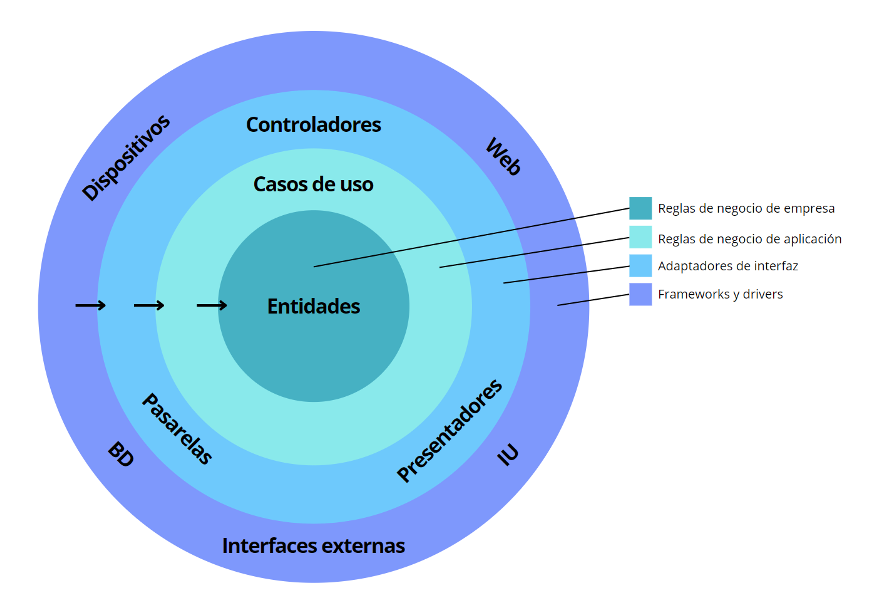
\includegraphics[width=0.7\textwidth]{img/manual/arquitectura_hexagonal.png}
    \caption{Arquitectura hexagonal.} \label{Img:Arquitectura+Hexagonal}
\end{figure} 

La arquitectura hexagonal permite que los sistemas puedan gozar de: a) independencia de frameworks, lo que implica que no depende de una biblioteca de software, sino que más bien puede utilizarlos como herramientas; y b) independencia de la IU, de la base de datos o de cualquier agente externo, lo que implica que el sistema puede ponerse a prueba sin necesidad de cualquiera de estos elementos, u otros, al mismo tiempo que puede cambiar fácilmente de interfaz, de servidor, o de cualquier otro agente externo que necesite. Lo anterior significa que la arquitectura hexagonal ofrece versatilidad al sistema y facilita su adaptabilidad a cualquier entorno de software \cite{book:arquitectura_limpia}. 

En este sentido, las entidades hacen referencia al objeto que establece las reglas del negocio, es decir, las reglas generales que dictan el funcionamiento del sistema. Los casos de uso son reglas de la aplicación más especificas que las anteriores; los adaptadores de interfaz son los encargados de convertir los datos provenientes de la interfaz al formato más conveniente para las dos capas anteriores. En la capa de frameworks y drivers se encuentran herramientas como la base de datos y el framework web, siendo la capa con los detalles menos relevantes que se mantienen en el exterior \cite{book:arquitectura_limpia}. Es importante considerar la regla de la dependencia, la cual estipula que los círculos más externos dependen de los internos y no al contrario, es decir, de adentro hacia afuera cada capa depende de la anterior.

En base a lo precedentemente expuesto amerita explicitar que la selección de la arquitectura hexagonal para el presente proyecto se motivó en que ésta permite el desacoplamiento de la lógica de negocio y las interfaces externas. Esto significa que se puede cambiar la base de datos, interfaz o invocaciones a APIs externas para la misma lógica de negocio, sin alterarla esencialmente. Ello asegura una escalabilidad y mantenibilidad de 
\emph{RedEM} a futuro. Habilitando a modificar, actualizar o reemplazar las partes individuales de la aplicación sin tener que reescribir todo el sistema, me centrarme en la implementación y no en otras capas del mismo. Por último, pero no menos importante, es una arquitectura con la que no tenía experiencia previa y quería desafiarme a aprenderla tanto académicamente como para aplicarla a nivel laboral.


\section{Control de versiones}
\begin{itemize}
\tightlist
\item
  Herramientas consideradas:
  \href{https://git-scm.com/}{Git} y
  \href{https://subversion.apache.org/)}{Subversion (SVN)}.
\item
  Herramienta elegida: \href{https://git-scm.com/}{Git}.
\end{itemize}
Se utilizó Git ya que este ofrece un modelo de ramificación y fusión más avanzado que SVN, lo que permite a los desarrolladores trabajar en paralelo en diferentes características o correcciones de errores sin interferir entre sí \cite{art:pro_git}. Asimismo, SVN consume más recursos a nivel de memoria por tener un sistema de guardado menos eficiente que el de Git. Además, es de considerar que al día de hoy el uso de Git proporciona integración con diferentes herramientas.

\subsection{Gestión del proyecto}
\begin{itemize}
\tightlist
\item
  Herramientas consideradas:
  \href{https://github.com/features/issues}{Github Projects},
  \href{https://trello.com/home)}{Trello} y \href{https://www.atlassian.com/es/software/jira}{Jira}.
\item
  Herramienta elegida: \href{https://www.atlassian.com/es/software/jira)}{Jira}.
\end{itemize}
Las ventajas de JIRA incluyen la capacidad de rastrear y solucionar problemas y tareas de manera eficiente, la personalización de flujos de trabajo y la integración con otras herramientas de Atlassian como Confluence y Bitbucket \cite{art:jira_osman}. De igual forma, posee una interfaz amigable que facilita el seguimiento del proyecto en tiempo real y, a diferencia de otras herramientas, permite tener un flujo de desarrollo de software más adaptado a los estándares de la industria ofreciendo métricas más adecuadas para la evaluación del desarrollo del proyecto, como su velocidad. Asimismo tengo conocimiento de esta herramienta por experiencia laboral.

\subsection{Editor del código}
\begin{itemize}
\tightlist
\item
  Herramientas consideradas:
  \href{https://code.visualstudio.com/}{Visual Studio Code} y 
  \href{https://www.jetbrains.com/go/)}{Goland}.
\item
  Herramienta elegida: \href{https://code.visualstudio.com/}{Visual Studio Code}.
\end{itemize}
Visual Studio Code es un editor de código de fuente abierto, gratuito, y multiplataforma con una gran cantidad de extensiones disponibles, y que se utiliza para desarrollar aplicaciones en una variedad de lenguajes de programación como C, C\#, Java, Python, JavaScript, TypeScript, Golang, entre otros \cite{art:visual_code_flores}. En este sentido, no se requirió de licencia para el editor de código facilitando su uso.

\subsection{Procesador de texto \LaTeX}
\begin{itemize}
\tightlist
\item
  Herramientas consideradas:
  \href{https://www.latex-project.org/}{LATEX} y 
  \href{https://www.microsoft.com/en-ww/microsoft-365/word)}{MS Word}.
\item
  Herramienta elegida: \href{https://www.latex-project.org/}{LATEX}.
\end{itemize}
\LaTeX{} es un lenguaje de marcado utilizado para la creación de documentos científicos y técnicos. En este sentido, se decidió trabajar con \LaTeX{} en el presente proyecto debido a su alta calidad tipográfica, la facilidad para crear fórmulas matemáticas complejas, la capacidad de automatizar la creación de tablas e índices\cite{art:latex}. Fue, asimismo, un desafío ya que no conocía esta herramienta para la elaboración de documentos y decidi acercarme a ella.


\subsection{Calidad del Código}
\begin{itemize}
\tightlist
\item
  Herramientas consideradas:
  \href{https://www.sonarsource.com/products/sonarqube/}{SonarQube} y 
  \href{https://circleci.com/)}{CircleCI}.
\item
  Herramienta elegida: \href{https://www.sonarsource.com/products/sonarqube/}{SonarQube}.
\end{itemize}
SonarQube es una plataforma gratuita de análisis de código abierto que permite evaluar la calidad del código fuente de los proyectos. Esta herramienta está diseñada para identificar y corregir errores de programación, vulnerabilidades de seguridad, patrones de diseño ineficientes y otros problemas comunes que pueden afectar la calidad del código \cite{art:sonarqube_ortega}. Se seleccionó esta herramienta puesto que ofrece informes detallados y personalizables sobre la calidad del código y es compatible con una amplia variedad de lenguajes de programación, como Golang, además de que puede integrarse con Github para obtener información detallada sobre la calidad del código. Asimismo, puede ser instalado en un servidor para ejecutar pruebas, sin pagar licencia por uso, pudiendo ser implementado en proyectos comerciales.


\subsection{Integración Continúa}
\begin{itemize}
\tightlist
\item
  Herramientas consideradas:
  \href{https://www.sonarsource.com/products/sonarqube/}{Github Actions} y 
  \href{https://circleci.com/)}{Jenkins}.
\item
  Herramienta elegida: \href{https://www.sonarsource.com/products/sonarqube/}{Github Actions}.
\end{itemize}
Github Actions es una plataforma que permite automatizar la compilación, prueba y despliegue de un código gracias a su característica de integración y despliegue continuo. Permite hacer despliegues en el servidor, releases, liberar versiones, y tener una mayor cantidad de usuarios por cuenta compartida. Además, tiene una herramienta que permite hacer Gitflow (manejo de branches), lo que facilita la gestión del desarrollo del software. Así, Github Actions permite reducir las acciones requeridas para ejecutar el código a través de la creación de un flujo de trabajo (Canorea, 2021). Se eligió Github Actions por su integración con Github y por el hecho de no necesitar de un hosting propio para ser instalado \cite{art:github_actions}

\subsection{Gestor de base de datos}
\begin{itemize}
\tightlist
\item
  Herramientas consideradas:
  \href{https://tableplus.com/}{TablePlus} y 
  \href{https://www.pgadmin.org/)}{pgAdmin}.
\item
  Herramienta elegida: \href{https://tableplus.com/}{TablePlus}.
\end{itemize}
TablePlus es un software de gestión de bases de datos, que fue seleccionado para el presente proyecto por su interfaz gráfica de usuario intuitiva y fácil de usar, que permite a los usuarios conectarse y administrar múltiples bases de datos de manera eficiente y en una sola aplicación y navegar por bases de datos relacionales de forma cómoda y sencilla \cite{art:tableplus}. Ofrece una serie de características útiles como la de autocompletado código SQL, la búsqueda de texto completo y la vista de schema, que hacen que la gestión de bases de datos sea más eficiente y productiva.

\subsection{Herramientas de diagrama}
\begin{itemize}
\tightlist
\item
  Herramientas consideradas:
  \href{https://draw.io/}{Draw.io} y 
  \href{https://www.lucidchart.com/)}{Lucid Chart}.
\item
  Herramienta elegida: \href{https://draw.io/}{Draw.io}.
\end{itemize}
Es útil para diseñar diagramas de flujo, de procesos, organigramas, diagramas de red, UML, e incluso mapas conceptuales. Posee una interfaz de usuario fácil de manejar y entender basada en la función de arrastrar y soltar, y elementos básicos como flechas, formas, imágenes y demás.
Se eligió esta plataforma para el presente proyecto por su simplicidad y familiaridad con el software. \cite{art:draw_io}

\subsection{Hosting del Proyecto}

\subsubsection{Servidor}
\begin{itemize}
\tightlist
\item
  Herramientas consideradas:
  \href{https://www.digitalocean.com/}{Digital Ocean} y 
  \href{https://aws.amazon.com/es/)}{Amazon AWS}.
\item
  Herramienta elegida: \href{https://www.digitalocean.com/}{Digital Ocean}.
\end{itemize}
Digital Ocean es una plataforma de alojamiento en la nube que ofrece la posibilidad de crear y administrar maquinas virtuales, así como otros servicios relacionados con la infraestructura en la nube; proporciona un entorno seguro y escalable para la implementación de aplicaciones web y móviles \cite{art:digital_ocean}. En este sentido, se eligió Digital Ocean por ser costo-efectivo más conveniente.

\subsubsection{Base de Datos DBaaS (Database as a Service)}
\begin{itemize}
\tightlist
\item
  Herramientas consideradas:
  \href{https://www.digitalocean.com/products/managed-databases}{PostgreSQL Digital Ocean} y 
  \href{https://aws.amazon.com/es/rds/)}{PostgreSQL Amazon}.
\item
  Herramienta elegida:   \href{https://www.digitalocean.com/}{PostgreSQL Digital Ocean}.
\end{itemize}
Digital Ocean también provee alojamiento de base de datos como servicio, con los beneficos de ser altamente escalable, de fácil configuración y mantenimiento, asi como por ofrecer alta disponibilidad dentro de su precio mensual.
Si bien en la comparativa el precio de Amazon AWS era de 24 USD al mes, contra de 33.28 USD de Digital Ocean, se eligió este último a fin de mantener dentro de un mismo ecosistema tanto el hosting como el alojamiento de la base de datos y así no afectará la latencia.